%% Template de Trabalho de  Conclusão de Curso da Engenharia de Controle e Automação

\documentclass[
	12pt,				% tamanho da fonte
	openright,			% capítulos começam em pág ímpar (insere página vazia caso preciso)
	oneside,			% para impressão somente em um lado da folha.
%	twoside,			% para impressão em verso e anverso. Oposto a oneside
	a4paper,			% tamanho do papel. 
	% -- opções da classe abntex2 --
	chapter=TITLE,		% títulos de capítulos convertidos em letras maiúsculas
%	section=TITLE,		% títulos de seções convertidos em letras maiúsculas
	%subsection=TITLE,	% títulos de subseções convertidos em letras maiúsculas
	%subsubsection=TITLE,% títulos de subsubseções convertidos em letras maiúsculas
	% -- opções do pacote babel --
	english,			% idioma adicional para hifenização
	brazil				% o último idioma é o principal do documento
	]{abntex2temp} % classe abntex2ufop para escrita de trabalhos academicos

% ---
% Pacotes básicos 
% ---
%\usepackage{lmodern}			% Usa a fonte Latin Modern	
\usepackage{times}				% Usa a fonte Latin Modern	
\usepackage{fancyvrb}			% Para mudança de fonte ambiente verbatim
\DefineVerbatimEnvironment{verbatim}{Verbatim}{fontfamily=zi4}
\usepackage[T1]{fontenc}		% Selecao de codigos de fonte.
\usepackage[utf8]{inputenc}		% Codificacao do documento (conversão automática dos acentos)

\usepackage{lastpage}			% Usado pela Ficha catalográfica
\usepackage{indentfirst}		% Indenta o primeiro parágrafo de cada seção.
\usepackage{color}				% Controle das cores
\usepackage{graphicx}			% Inclusão de gráficos
\usepackage{microtype} 			% para melhorias de justificação
\usepackage{supertabular}       % tabela na capa do documento
% ---
		
% ---
% Pacotes adicionais, usados apenas no âmbito do Modelo Canônico do abnteX2 - pode ser removido

% ---
% Pacotes adicionais, usados no anexo do modelo de folha de identificação
% ---
\usepackage{multicol}
\usepackage{multirow}
\usepackage{lipsum}				% para geração de dummy text
% ---

% ---
% Pacotes de citações
% ---
\usepackage[brazilian,hyperpageref]{backref}	 % Paginas com as citações na bibliografia
\usepackage[alf]{abntex2cite}	% Citações padrão ABNT 6023

% --- 
% CONFIGURAÇÕES DE PACOTES
% --- 

% ---
% Configurações do pacote backref
% Usado sem a opção hyperpageref de backref
\renewcommand{\backrefpagesname}{Citado na(s) página(s):~}
% Texto padrão antes do número das páginas
\renewcommand{\backref}{}
% Define os textos da citação
\renewcommand*{\backrefalt}[4]{
	\ifcase #1 %
		Nenhuma citação no texto.%
	\or
		Citado na página #2.%
	\else
		Citado #1 vezes nas páginas #2.%
	\fi}%
% ---

% ---
% Informações de dados para CAPA e FOLHA DE ROSTO
% ---
\titulo{INSERIR TÍTULO DO TRABALHO}
\autor{NOME DO AUTOR}
\local{Ouro Preto}
\data{2019}
\orientador{Prof. Nome do Primeiro Orientador, Ph.D.}
\coorientador{Prof. Nome do Segundo Orientador, Dr.Sc.}
\instituicao{Universidade Federal de Ouro Preto}
\unidade{Escola de Minas}
\colegiado{Colegiado do curso de Engenharia de Controle e Automa{\c c}{\~a}o - CECAU}
\tipotrabalho{Monografia de Gradua{\c c}{\~a}o em Engenharia de Controle e Automa{\c c}{\~a}o }
% O preambulo deve conter o tipo do trabalho, o objetivo, 
% o nome da instituição e a área de concentração 
\preambulo{Monografia apresentada ao Curso de Engenharia de Controle e Automa{\c c}{\~a}o da Universidade Federal de Ouro Preto como parte dos requisitos para a obten{\c c}{\~a}o do Grau de Engenheiro de Controle e Automa{\c c}{\~a}o.}
% ---


% ---
% Configurações de aparência do PDF final

% alterando o aspecto da cor azul
\definecolor{blue}{RGB}{41,5,195}

% informações do PDF
\makeatletter
\hypersetup{
     	%pagebackref=true,
		pdftitle={\@title}, 
		pdfauthor={\@author},
    	pdfsubject={\imprimirpreambulo},
	    pdfcreator={LaTeX with abnTeX2},
		pdfkeywords={abnt}{latex}{abntex}{abntex2}{trabalho acadêmico}, 
		colorlinks=true,       		% false: boxed links; true: colored links
    	linkcolor=blue,          	% color of internal links
    	citecolor=blue,        		% color of links to bibliography
    	filecolor=magenta,      		% color of file links
		urlcolor=blue,
		bookmarksdepth=4
}
\makeatother
% --- 

% --- 
% Espaçamentos entre linhas e parágrafos 
% --- 

% O tamanho do parágrafo é dado por:
\setlength{\parindent}{1.3cm}

% Controle do espaçamento entre um parágrafo e outro:
\setlength{\parskip}{0.2cm}  % tente também \onelineskip

% ---
% compila o indice
% ---
\makeindex
% ---

% ----
% Início do documento
% ----
\begin{document}

% Retira espaço extra obsoleto entre as frases.
\frenchspacing 

% ------------------------------------------
% ELEMENTOS PRÉ-TEXTUAIS
% ------------------------------------------
% \pretextual

% ---
% Capa
% ---
\imprimircapa
% ---

% ---
% Folha de rosto
% (o * indica que haverá a ficha bibliográfica)
% ---
\imprimirfolhaderosto*
% ---

% ---
% Inserir a ficha bibliografica
% ---

% Isto é um exemplo de Ficha Catalográfica, ou ``Dados internacionais de
% catalogação-na-publicação''. 
% Porém, a biblioteca da sua universidade lhe fornecerá um PDF
% com a ficha catalográfica definitiva após a defesa do trabalho. Quando estiver
% com o documento, salve-o como PDF no diretório do seu projeto e substitua todo
% o conteúdo de implementação deste arquivo pelo comando abaixo que está comentado 
% (nao se esqueça de comentar o antigo ambiente de ficha catalográfica):
%
% \begin{fichacatalografica}
%     \includepdf{fig_ficha_catalografica.pdf}
% \end{fichacatalografica}
%
%
% Ou, você poderá também ler os dados da ficha e adicionar no póprio código
% como as palavras-chave, CDU e dimensões do trabalho: 
\begin{fichacatalografica}
	\vspace*{\fill}					% Posição vertical
	\hrule							% Linha horizontal
	\begin{center}					% Minipage Centralizado
	\begin{minipage}[c]{12.5cm}		% Largura
	
	\imprimirautor
	
	\hspace{0.5cm} \imprimirtitulo  / \imprimirautor. --
	\imprimirlocal, \imprimirdata-
	
	\hspace{0.5cm} \pageref{LastPage} p. : il. (algumas color.) ; 30 cm.\\
	
	\hspace{0.5cm} \imprimirorientadorRotulo~\imprimirorientador\\
	
	\hspace{0.5cm}
	\parbox[t]{\textwidth}{\imprimirtipotrabalho~--~\imprimirinstituicao,
	\imprimirdata.}\\
	
	\hspace{0.5cm}
		1. Palavra-chave1.
		2. Palavra-chave2.
		I. Orientador.
		II. Universidade xxx.
		III. Faculdade de xxx.
		IV. Título\\ 			
	
	\hspace{8.75cm} CDU 02:141:005.7\\
	
	\end{minipage}
	\end{center}
	\hrule
\end{fichacatalografica}
% ---

% ---
% Inserir folha de aprovação
% ---

% Isto é um exemplo de Folha de aprovação, elemento obrigatório da NBR
% 14724/2011 (seção 4.2.1.3). Você pode utilizar este modelo até a aprovação % do trabalho. Após isso, substitua todo o conteúdo deste arquivo por uma % imagem da página assinada pela banca com o comando abaixo:
%
% \includepdf{folhadeaprovacao_final.pdf}
%
\begin{folhadeaprovacao}
% 
   Monografia intitulada INSERIR TÍTULO DO TRABALHO defendida e aprovada em $XX$ de $XX$ de \imprimirdata, pela comiss{\~a}o avaliadora constitu{\'i}da pelos professores:
   \vspace*{\fill}
   \assinatura{\textbf{\imprimirorientador} \\ Orientador} 
   \vspace*{\fill}
   \assinatura{\textbf{Prof. Dr. Nome do Convidado 1} \\ Convidado}
   \vspace*{\fill}
   \assinatura{\textbf{Prof. Dr. Nome do Convidado 2} \\ Convidado}
   \vspace*{\fill}
   %\assinatura{\textbf{Professor} \\ Convidado 3}
  % \vspace*{\fill}
   %\assinatura{\textbf{Professor} \\ Convidado 4}
  % \vspace*{\fill}
      
   \begin{center}
    \vspace*{0.5cm}
    {\large\imprimirlocal}, {\large\imprimirdata}
    \vspace*{1cm}
  \end{center}
  
\end{folhadeaprovacao}
% ---

% ---
% Dedicatória
% ---
\begin{dedicatoria}
   \vspace*{\fill}
   \flushright
   \noindent
   \textit{ Este trabalho é dedicado às crianças adultas que,\\
   quando pequenas, sonharam em se tornar cientistas.} \vspace*{\fill}
\end{dedicatoria}
% ---

% ---
% Agradecimentos
% ---
\begin{agradecimentos}
\noindent Inserir aqui seus agradecimentos.

\end{agradecimentos}
% ---

% ---
% Epígrafe
% ---
\begin{epigrafe}
    \vspace*{\fill}
	\begin{flushright}
		\textit{``Matéria é a parte acidental.'' (Oliver Lodge)}
	\end{flushright}
\end{epigrafe}
% ---

% ---
% RESUMOS
% ---

% resumo em português
\setlength{\absparsep}{18pt} % ajusta o espaçamento dos parágrafos do resumo
\begin{resumo}
 \noindent É a apresentação dos pontos relevantes de um documento. Deve ser redigido em parágrafo único, com verbo na voz ativa e na 3a pessoa do singular, com frases de ordem direta, evitando-se explicações repetitivas, abreviaturas, siglas e fórmulas. O resumo deve conter a motivação, a justificativa, o método principal utilizado, resultados mais relevantes e conclusão. Extensão recomendada aos resumos: 150 a 500 palavras.

 \textbf{Palavras-chaves}: palavra1. palavra2. palavra3.
\end{resumo}

% resumo em inglês
\begin{resumo}[Abstract]
 \begin{otherlanguage*}{english}

\noindent This is the english abstract.

   \vspace{\onelineskip}
 
   \noindent 
   \textbf{Key-words}: word1. word2. word3.
 \end{otherlanguage*}
\end{resumo}

% ---
% inserir lista de figuras
% ---
\pdfbookmark[0]{\listfigurename}{lof}
\listoffigures*
\cleardoublepage
% ---

% ---
% inserir lista de tabelas
% ---
\pdfbookmark[0]{\listtablename}{lot}
\listoftables*
\cleardoublepage
% ---

% ---
% inserir lista de abreviaturas e siglas
% ---
\begin{siglas}
  \item[ABNT] Associação Brasileira de Normas Técnicas
  \item[abnTeX] ABsurdas Normas para TeX
\end{siglas}
% ---

% ---
% inserir lista de símbolos
% ---
\begin{simbolos}
  \item[$ \Gamma $] Letra grega Gama
  \item[$ \Lambda $] Lambda
  \item[$ \zeta $] Letra grega minúscula zeta
  \item[$ \in $] Pertence
\end{simbolos}
% ---

% ---
% inserir o sumario
% ---
\pdfbookmark[0]{\contentsname}{toc}
\tableofcontents*
\cleardoublepage
% ---

% ------------------------------------------
% ELEMENTOS TEXTUAIS
% ------------------------------------------
\textual
\pagestyle{simple}

% ---
% Capítulos
% ---
\chapter[Introdução]{Introdução}

\section{Estado da arte}

Assuntos relevantes a temática da pesquisa proposta, com base em publicações técnicas e científicas, sobretudo artigos científicos nacionais e internacionais.   \cite{doxiadis1965}

\section{Objetivos gerais e específicos}

\section{Justificativa do trabalho}

\section{Estrutura do trabalho}


\chapter{Revisão da literatura}

Neste capítulo é realizada uma fundamentação de toda a teoria necessária para a compreensão do trabalho desenvolvido. Os temas estão divididos em forma de tópicos e cada tópico apresenta conceitos e definições encontradas na literatura e que foram utilizadas ao longo do projeto. 

\section{Robótica Móvel}
A robótica móvel é uma das grandes áreas da robótica. Robôs são, por definição, manipuladores ou mecanismos reprogramáveis e multifuncionais utilizados para mover materiais, ferramentas ou partes através de diferentes trajetórias definidas e para realização de diversas tarefas. A principal diferença entre os robôs manipuladores, amplamente aplicados em industrias, e robôs móveis é que o primeiro tipo realiza movimentos dentro de um espaço de trabalho definido e o segundo consegue se locomover no espaço, seja utilizando rodas, pés ou outro meio de locomoção. \cite{nehmzow2012mobile}
\par
Na literatura, é possível encontrar diversas classificações para os robôs móveis. Uma delas é a divisão por meio de locomoção do robô, que pode ser terrestre, aquática, aérea ou hibrida. Uma das características presentes em todas as classificações de locomoção é a ideia da biomimética, ou seja, a movimentação dos robôs é sempre inspirada na fisiologia e nos métodos de locomoção encontradas nos animais. \cite{russo2020survey} Dentro da classificação por meio de locomoção é possível realizar uma subdivisão pela forma com que esse movimento será realizada. Por exemplo, robôs terrestres podem se locomover através de pernas, rodas, peristaltismo, deslizamento, braquiação e adesão a superfícies. \cite{russo2020survey}
\par
Dentro do subgrupo de robôs móveis terrestres que utilizam rodas, também é possível realizar um agrupamento de acordo com a disposição, tração exercida e grau de mobilidade que a roda possui. As rodas podem ser do tipo mecano, uma roda omnidirecional, caster, fixas ou dirigida. O número e o tipo dessas rodas define o grau de liberdade que o robô possui. \cite{gruber2016} 
\subsection{Autonomia de Robôs Móveis}

Também é possível realizar a classificação de robôs móveis conforme a sua autonomia em relação a necessidade de intervenção humana para a realização de tarefas. Os robôs podem ser classificados como:
\begin{itemize}
    \item Tele-operado: Existe a necessidade de um operador humano que fará o controle da movimentação do robô com o auxilio de câmeras e outros sensores. Neste caso o é incapaz de realizar tarefas por conta própria.
    \item Semiautônomo: O robô possui capacidade de se movimentar sem o auxílio do operador, mas essa movimentação é limitada à algumas funções e, de forma geral, existe a necessidade de acompanhamento e atuação humana para garantir o cumprimento de objetivos;
    \item Autônomo: São robôs projetados para atuar sem auxílio humano, conseguem realizar as tarefas para as quais foram projetos de forma independente. Robôs autônomos se utilizam de diversos sensores, câmeras e outras ferramentas de instrumentação para conseguirem captar as informações do ambiente e depois realizam um planejamento de ações com base em técnicas de inteligencia artificial, conseguindo determinar quais os passos necesários para cumprir o objetivo. 
\end{itemize}

\subsection{Robô Diferencial}
De acordo com \citeonline{dudek2010computational}, robôs diferenciais são uma classe de robôs móveis que possuem duas rodas motorizadas que são conectadas através de um mesmo eixo. As rodas, por possuírem motorização independente, podem aplicar diferentes torques e assim permitir que o robô realize distintos movimentos de rotação tanto para frente quanto para trás. 
\par
Robôs diferenciais podem possuir variações em sua estrutura, podendo possuir rodas do tipo caster para auxiliar na estabilidade do sistema, assim como também podem possuir mais eixos motorizados trabalhando em conjunto. \cite{guarino1995}
\par

\subsubsection{Cinemática}
Uma das configurações possíveis, é o robô com duas rodas diferenciais no eixo traseiro e uma roda passiva do tipo caster no centro dianteiro. Estes robôs são conhecidos como uniciclos. \cite{aicardi1995closed}
\par
A cinemática desses robôs pode ser descrita de forma planar, através de coordenadas cartesianas. Como pode ser visto na Figura \ref{fig:robo_coordenada_cart}, a posição do robô pode ser dada através de um ponto central nos eixos $(x,y)$ e sua orientação pode ser obtido de um ângulo $\theta$. \cite{sousa2003controle}
\par

\begin{figure}[ht]
    \centering
    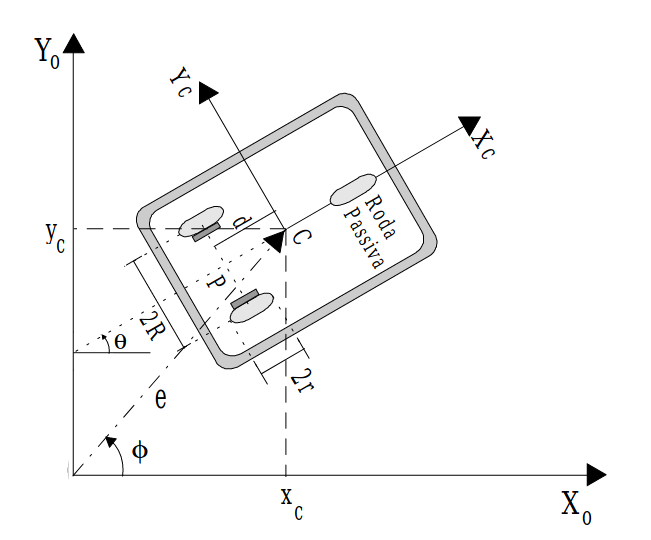
\includegraphics[width=0.8\textwidth]{capitulos/robo_dif_coordenadas.png}
    \caption{Robô diferencial em sistema de coordenadas cartesianas. \cite{sousa2003controle}}
    \label{fig:robo_coordenada_cart}
\end{figure}
\begin{figure}[ht]
    \centering
    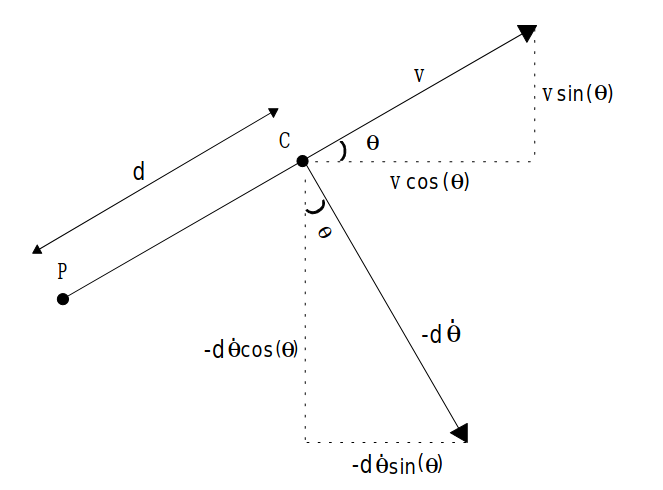
\includegraphics[width=0.8\textwidth]{capitulos/robo_dif_vetorial.png}
    \caption{Diagrama vetorial do robô diferencial, mostrando os vetores de velocidade. \cite{sousa2003controle}}
    \label{fig:robo_coordenada_vet}
\end{figure}
Ampliando a visão do modelo cinemático, pode-se visualizar a equação que rege as velocidades do robô diferencial através da Figura \ref{fig:robo_coordenada_vet}. Podemos escrever a equação através de:
\begin{equation}
  \begin{cases}
     \dot{x_{c}} = cos(\theta)v - dsin(\theta)\omega\\
     \dot{y_{c}} = sin(\theta)v + dcos(\theta)\omega\\
     \dot{\theta} = \omega
  \end{cases}
  \label{eq:1}
\end{equation},
ou, em forma matricial
\begin{equation}
    \begin{bmatrix}
       \dot{x_{c}} \\
       \dot{y_{c}} \\
       \dot{\theta}
     \end{bmatrix} = \begin{bmatrix}
       cos(\theta) & -dsin(\theta)\\
        sin(\theta) & dcos(\theta)\\
       0 & 1
     \end{bmatrix}\begin{bmatrix}
       v\\
       \omega\\
     \end{bmatrix}
     \label{eq:2}
\end{equation},
onde $v$ é a velocidade linear e $\omega$ a velocidade angular. \cite{sousa2003controle}
Com o modelo apresentado na Equação \ref{eq:2} é possível realizar o controle das variáveis de saída, $v$ e $w$, de acordo com os parâmetros de entrada que indicam a posição do robô $x, y$ e $\theta$.
\par
Outra forma de representar a cinemática direta de um robô diferencial é utilizando coordenadas polares. \cite{aicardi1995closed} Onde a representação cartesiana pode ser transformada nas variáveis $(e, \phi, \alpha)$ que podem ser descritas por:
\begin{equation}
  \begin{cases}
     e = \sqrt{x_{c}^2 + y_{c}^2}\\
     \phi = arctan2(y_{c},x_{c})\\
     \alpha = \theta - \phi
  \end{cases}
  \label{eq:3}
\end{equation}
e também, $x_{c} e y_{c}$ podem ser escritos como:
\begin{equation}
  \begin{cases}
     x_{c} = e cos(\phi)\\
     y_{c} = esin(\phi)\\
  \end{cases}
  \label{eq:4}
\end{equation}
Desta forma, é possível realizar o controle através dos parâmetros $e$, que representa o módulo da posição do robô e o parâmetro $\alpha$, que representa a orientação do robô em relação ao eixo cartesiano definido pelo sistema.
\section{Controle PID}
O algoritmo de controle PID é utilizado em larga escala para processos que necessitem de controle por realimentação, sejam eles industriais, residenciais ou afins. \cite{astrom1995}
\par
\subsection{Controle Realimentado}
O PID funciona através do principio de realimentação, que pode ser definido como: "O acréscimo da variável manipulada quando a variável de processo é menor do que o setpoint e o decréscimo da variável manipulada quando a variável de processo é maior do que o setpoint."  Utilizando este princípio, vários modelos de controladores foram criados, sendo o mais simples deles o controle on-off, que possui um sinal de controle discreto de ligado ou desligado, e o mais utilizado sendo o PID. \cite{astrom1995}

\begin{figure}[ht]
    \centering
    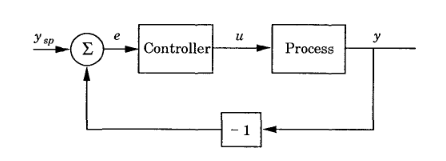
\includegraphics[width=0.8\textwidth]{capitulos/processo_feedback.png}
    \caption{Diagrama de blocos de um processo realimentado simples. \cite{astrom1995}}
    \label{fig:processo_feedback}
\end{figure}
\subsection{Elemento Proporcional, Integral e Derivativo de um PID}
Um controlador PID pode ser dividido em três partes: Proporcional, integral e derivativa. Cada uma destas partes possui uma influência em como o controlador vai alterar a resposta do sistema. \cite{ogata2011engenharia} Nesta seção cada uma delas será discutida de forma separada.
\subsubsection{Parte Proporcional}
A parte proporcional do controlador pode ser descrita pela equação: 
\begin{equation}
    u(t) = K e(t)
\end{equation}
Onde o sinal de saída $u(t)$ é proporcional ao sinal de erro $e(t)$ junto a um ganho $K$, chamado de ganho proporcional. Ou seja, o controlador proporcional apenas amplifica o sinal de controle em relação ao erro. \cite{ogata2011engenharia}

\begin{figure}[ht]
    \centering
    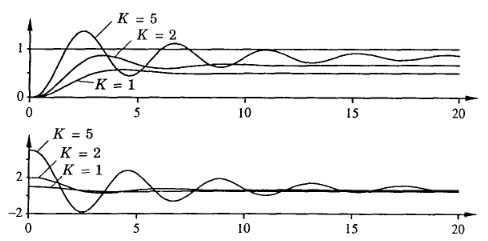
\includegraphics[width=0.8\textwidth]{capitulos/acao_controle_proporcional.png}
    \caption{Gráfico demonstrando o sinal de saída de um controlador proporcional com diferentes valores de K. \cite{astrom1995}}
    \label{fig:acao_controle_proporcional}
\end{figure}
\subsubsection{Parte Integral}
A ação integral do controlador tem a função de realizar uma somatória dos erros do sistema afim de permitir que o mesmo, em regime permanente, seja zerado.\cite{ogata2011engenharia} Sua equação é:
\begin{equation}
    u(t) = K_{i} \int_0^t e(t) dx
\end{equation}
Onde $K_{i}$ é um ganho ajustável.

\begin{figure}[ht]
    \centering
    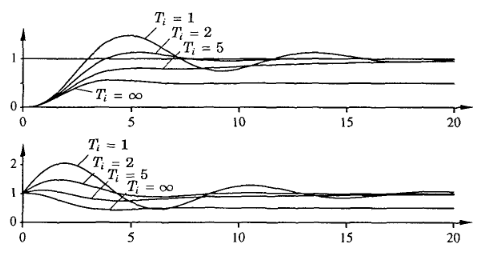
\includegraphics[width=0.8\textwidth]{capitulos/acao_controle_integral.png}
    \caption{Gráfico demonstrando o sinal de saída de um controlador integral com diferentes valores de $K_{i}$. \cite{astrom1995}}
    \label{fig:acao_controle_integral}
\end{figure}
\subsubsection{Parte Derivativa}
Já a parte derivativa possui o objetivo de realizar a previsão do erro que acontece no controlador, diminuindo o tempo que o sistema leva para se estabilizar.\cite{ogata2011engenharia} Sua componente é:
\begin{equation}
    u(t) = K_{d} \frac{de(t)}{dt}
\end{equation}

\begin{figure}[ht]
    \centering
    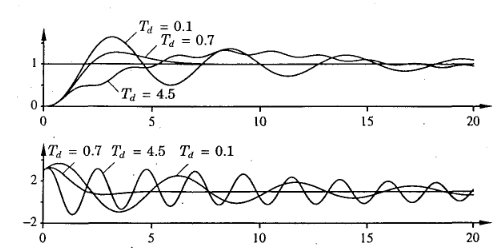
\includegraphics[width=0.8\textwidth]{capitulos/acao_controle_derivativo.png}
    \caption{Gráfico demonstrando o sinal de saída de um controlador derivativo com diferentes valores de $K_{d}$. \cite{astrom1995}}
    \label{fig:acao_controle_derivativo}
\end{figure}
\subsection{Controlador PID}
O controlador PID tradicional é a junção dos três termos citados acima, se tornando um controlador robustos para trabalhar com problemas que precisam possuir erro nulo em regime permanente e também chegar na estabilidade mais rapidamente.\cite{ogata2011engenharia} Ou seja, o PID tradicional é:
\begin{equation}
    u(t) = K_{p} e(t) + K_{i} \int_0^t e(t) dx + K_{d} \frac{de(t)}{dt}
\end{equation}
Cuja descrição em diagrama de blocos está demonstrada na Figura \ref{fig:representacao_pid}.
\begin{figure}[ht]
    \centering
    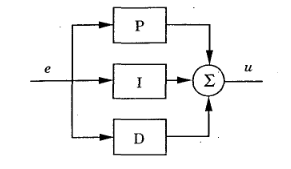
\includegraphics[width=0.5\textwidth]{capitulos/representacao_pid.png}
    \caption{Representação de diagrama de blocos de um controlador PID, separado por suas três componentes. \cite{astrom1995}}
    \label{fig:representacao_pid}
\end{figure}
\subsection{Sintonização de Controladores PID}
Para que o controlador PID consiga cumprir seu objetivo corretamente é muito importante que seus ganhos $K_{p}$, $K_{i}$ e $K_{d}$ sejam corretamente definidos. Esse projeto do controlador pode se utilizar de diversos métodos. Quando a planta é relativamente simples, sua função de transferência pode ser definida e métodos de analíticos de projetos podem ser utilizados. Entretanto, quando a planta envolve mais complexidade e não é possível separar de forma precisa a relação entre as variáveis físicas, deve-se realizar a sintonia através de regras definidas em literatura ou métodos numéricos, utilizadas inclusive em controladores PID inteligentes que conseguem realizar a sua própria sintonia fina de forma automática. \cite{ogata2011engenharia}
\par
Uma dos métodos de sintonia mais difundidas na literatura é o de  Ziegler-Nichols. O método se baseia no regime transitório da planta para encontrar o ganho proporcional $K_{p}$, o tempo integral $T_{i}$ e o tempo derivativo $T_{p}$. Esses parâmetros podem ser obtidos através da aplicação de um degrau unitário (Figura \ref{fig:resposta_degrau_unitario}  na entrada da planta e da análise na curva de resposta do sinal. Para a utilização do método, alguns critérios devem ser satisfeitos:
\begin{figure}[ht]
    \centering
    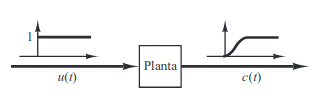
\includegraphics[width=0.5\textwidth]{capitulos/resposta_degrau_planta.png}
    \caption{Aplicação de um degrau unitário.\cite{ogata2011engenharia}}
    \label{fig:resposta_degrau_unitario}
\end{figure}
    \begin{itemize}
        \item A planta não poderá possuir integradores ou polos complexos conjugados dominantes.
        \item A resposta gráfica do sistema deverá aparentar possuir uma forma em S
    \end{itemize}
    Satisfeitos esses dois requisitos, é possível obter os valores de $L$, denominado atraso do sistema, e $T$, a constante de tempo. Essas duas constantes são obtidas através do tracejado da linha tangente à inflexão que ocorre na curva em S, vide Figura \ref{fig:curva_projeto_pid}, e identificando os pontos onde a linha cruza o eixo temporal e o eixo do ganho $K$. . 
    \begin{figure}[ht]
        \centering
        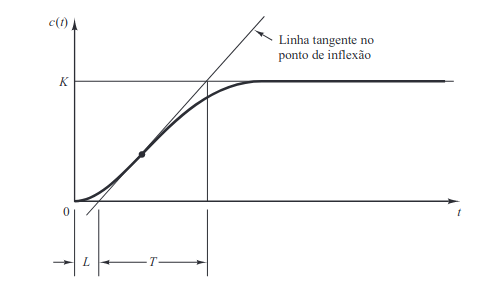
\includegraphics[width=0.5\textwidth]{capitulos/curva_projeto_pid.png}
        \caption{Análise da resposta ao degrau.\cite{ogata2011engenharia}}
        \label{fig:curva_projeto_pid}
    \end{figure}\par
    Através das duas constantes, Ziegler e Nichols propuseram a tabela \ref{tab:tabela_ziegler_nichols}, mostrada abaixo para encontrar os parâmetros $K_{p}$, $T_{i}$ e $T_{i}$.
    \begin{table}[h!]
        \centering
        \caption{Regra de Ziegler-Nichols}
        \begin{tabular}{| r | c | c | c |}
        \hline
            Tipo de controlador & $K_{p}$ & $T_{i}$ & $T_{d}$ \\
            \hline
            P & $\frac{T}{L}$ & $\infty$ & $0$ \\
            \hline
            PI & $0,9\frac{T}{L}$ & $\frac{L}{0,3}$ & $0$ \\
            \hline
            PID & $1,2\frac{T}{L}$ & $2L$ & $0,5L$ \\
        \hline
        \end{tabular}
        \label{tab:tabela_ziegler_nichols}
    \end{table}
    \par
    Desta forma, o controlador PID fica da forma
    \begin{equation}
        G_{c}(s)= K_{p} (1 + \frac{1}{T_{i}S} + T_{d}S)
    \end{equation}
\section{Visão Computacional}
Visão computacional é a área da ciência da computação que busca a interpretação de imagens, vídeos ou qualquer outro tipo de dado visual através de algoritmos. Seu objetivo é utilizar inteligência computacional para permitir que uma máquina consiga, da melhor forma possível, replicar elementos da visão humana. É considerada uma área ampla e difícil, por se tratar de um problema inverso, onde pesquisadores tentam obter informações através de um elemento visual que possui elementos a principio desconhecidos. Isso torna necessário a utilização de modelos físicos e técnicas de aprendizado de máquina. Mesmo assim, continua sendo um campo em expansão e em constante desenvolvimento. \cite{szeliski2021computer}
\subsection{Espaços de Cor}
Cores são elementos fundamentais na formação, manipulação e reconhecimento de imagens. Por conceito físico, as cores são formadas através de diferentes comprimentos de ondas que são captados pela retina humana e interpretas pelo cérebro.\par
\begin{figure}[ht]
    \centering
    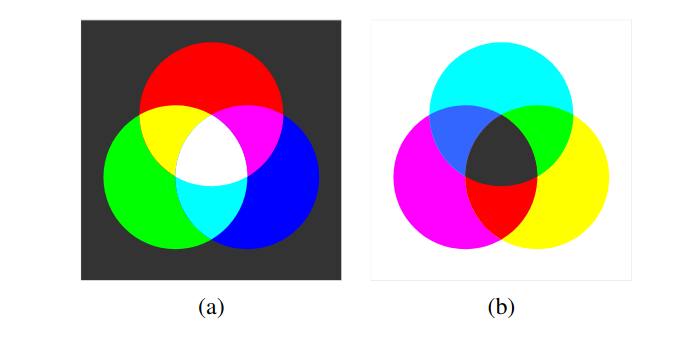
\includegraphics[width=0.8\textwidth]{capitulos/cores_adtivas_subtrativas.png}
    \caption{Formação de cores através dos métodos: (a) aditivos e (b) subtrativos.\cite{szeliski2021computer}}
    \label{fig:cores_adtivas_subtrativas}
\end{figure}
    
Em relação às imagens digitais, as cores podem ser representadas por diversos espaços, conhecidos como espaços de cores. CITAR Em uma câmera digital, os diferentes comprimentos de ondas são captados pelo sensor óptico e depois discretizados em três cores primárias: Azul, vermelho e verde, que, quando combinados de forma aditiva, conseguem representar todo o espectro de cores visíveis. Esse primeiro espaço de cores é conhecido como RGB e é muito utilizado para representação de cores em interfaces digitais. Nota-se que a utilização de três cores se deve ao fato da visão humana possuir três tipos de células, chamadas cones, que capturam diferentes comprimentos de onda da luz.\cite{szeliski2021computer}
\par
Outra forma de se representar as cores, também através da utilização de três primárias, é o espaço CMYB (Ciano, Magenta, Amarelo e Preto), que juntas conseguem formar outras cores do espectro visível através de subtração, conforme (Figura \ref{fig:cores_adtivas_subtrativas}).
\par
Outra característica importante, principalmente no processamento de imagens, é a interpolação entre cores. Ou seja, é possível agregar pixels que possuem apenas uma das cores primarias e armazenar a informação de qualquer outra cor criando uma nova matriz onde cada pixel contém informação das três cores.
\begin{figure}[ht]
    \centering
    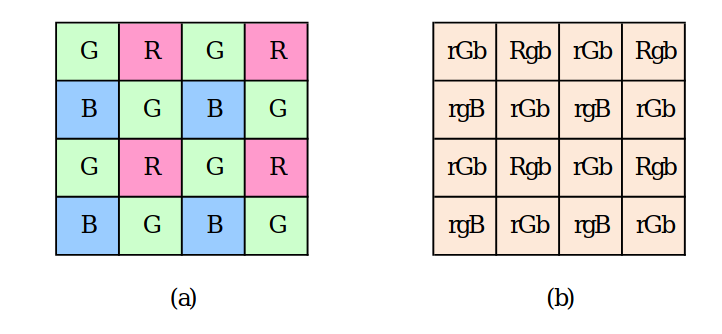
\includegraphics[width=0.8\textwidth]{capitulos/interpolacao_cores.png}
    \caption{Interpolação de cores. (a) Filtro com as cores primárias armazenadas de forma separada. (b) Matriz onde cada pixel armazena as três cores, gerados através de interpolação. \cite{szeliski2021computer}}
    \label{fig:interpolacao_cores}
\end{figure}
\par
Outra forma de representação das cores é através do espaço HSV. Esse espaço é interessante quando deseja-se filtrar um determinado intervalo de cores, pois permite agregar cores parecidas levando em consideração a iluminação do ambiente. De acordo com \citeonline{hall2012illumination},o espaço é formado através de um círculo de cores, que é representado pelo valor de hue (H), a saturação, ou intensidade de coloração, que é representado por (S) e o valor máximo de cor, que é representado por (V). A (Figura \ref{fig:cores_hsv}) é uma representação do espaço HSV.
\begin{figure}[ht]
    \centering
    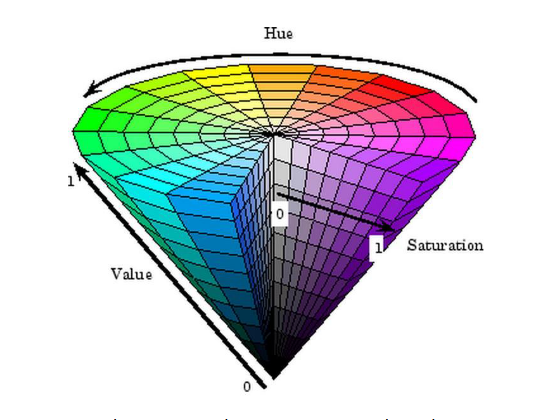
\includegraphics[width=0.8\textwidth]{capitulos/cores_hsv.png}
    \caption{Pirâmide HSV. \cite{erdogan2014shifting}}
    \label{fig:cores_hsv}
\end{figure}

\subsection{Operações Morfológicas}

Imagens binárias são matrizes formadas após uma operação de thresholding e podem ser utilizadas para diversas análises na área de visão computacional. Uma operação de thresholding normalmente é denotada da seguinte forma:
\begin{equation}
    \theta(f,t) = 
  \begin{cases}
    1       & \quad \text{if } f \geq t,\\
    0  & \quad \text{else}
  \end{cases}
    \label{eq:thresholding}
\end{equation}

De acordo com \citeonline{wilson2000handbook}, a forma mais comum de manipular imagens binárias é a de realizar operações morfológicas nas mesmas. O termo morfológico significa que a operação acaba por alterar a forma da imagem original. Para realizar as operações, é necessário realizar a convolução (Eq \ref{eq:morfologia_convolucao}) da imagem binária com algum elemento que servirá como filtro, seja ele uma matriz simples ou até mesmo formas mais complexas. A operação morfológica realizará uma busca e casamento de informações de acordo com o filtro estabelecido. \cite{szeliski2021computer}
\begin{equation}
    c = f \otimes s
    \label{eq:morfologia_convolucao}
\end{equation}
Onde $c$ é a convolução, $f$ a imagem binária e $s$ o filtro.
\par
As principais operações morfológicas são:
\begin{itemize}
    \item dilatação: $dilate(f,s) = \theta(c,1)$
    \item erosão: $erode(f,s) = \theta(c,S)$
    \item maioria: $majority(f,s) = \theta(c,S/2)$
    \item abertura: $open(f,s) = dilate(erode(f,s),s)$
    \item fechamento: $close(f,s) = erode(dilate(f,s),s)$
\end{itemize}
\begin{figure}[ht]
    \centering
    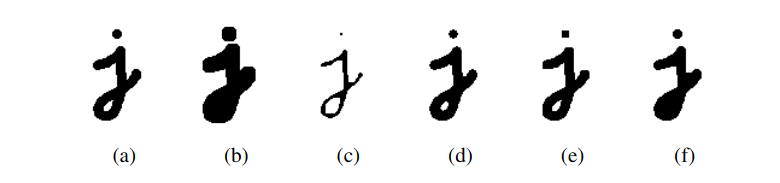
\includegraphics[width=0.8\textwidth]{capitulos/operacoes_morfologicas.png}
    \caption{(a) Imagem original, (b) Dilatação, (c) Erosão, (d) Maioria, (e) Abertura e (f) Fechamento. \cite{szeliski2021computer}}
    \label{fig:operacoes_morfologicas}
\end{figure}
Através da (Figura: \ref{fig:operacoes_morfologicas}) é possível visualizar o efeito de cada operação na imagem original. Esses efeitos são amplamente aplicados no reconhecimento de formas e padrões. 
\subsection{Bordas e Contornos}
No reconhecimento de padrões, conseguir identificar bordas e contornos de uma imagem é uma estratégia interessante e útil. Usualmente, esses elementos podem nos dar importantes informações acerca da imagem a ser processada, como diferentes formas, objetos e dados sobre a alocação desses itens no espaço tridimensional. \cite{szeliski2021computer}
\par
De forma qualitativa, bordas ocorrem em regiões da imagem onde existem diferenças de cor, intensidade ou textura. \cite{martin2004learning} Uma abordagem prática para definir as bordas é como um localização com rápida variação de cor ou intensidade. Para conseguir localizar de forma precisa e com o mínimo possível de ruídos utiliza-se, de forma mais comum, o filtro Gaussiano (Eq \ref{eq:filtro_gaussiano}), que permite remover ruídos da imagem e encontrar de forma mais precisa o que realmente é uma borda. \cite{szeliski2021computer}
\begin{equation}
    G(x,y,\sigma) = \frac{1}{2\pi\sigma^{2}}e^{-\frac{x^2+y^2}{2\sigma^2}}
    \label{eq:filtro_gaussiano}
\end{equation}
Para utilizar o filtro gaussiano com o objetivo de se obter as bordas de uma imagem é necessário que alguns passos algébricos sejam cumpridos, afim de se manipular a imagem e a obtenção de algumas informações relevantes. Uma dessas informações é a inclinação e direção da superfície com relação a sua intensidade. Essa inclinação pode ser obtida através do vetor gradiente $J(X)$, que é descrita como:
\begin{equation}
    J(X) = \nabla I(X) = (\frac{\partial I}{\partial x},\frac{\partial I}{\partial y})(X)
    \label{eq:borda_j}
\end{equation}
$J$ aponta na direção onde o crescimento da intensidade é maior. Manipulando as equações \ref{eq:filtro_gaussiano} e \ref{eq:borda_j} é possível encontrar um gradiente da imagem já filtrada, conforme a equação \ref{eq:borda_jsigma}

\begin{equation}
    J_{\sigma}(X) = \nabla [ G_{\sigma}(X) * I(X) ] = [\nabla G_{\sigma}](X) * I(X) 
    \label{eq:borda_jsigma}
\end{equation}

Entretanto, algumas aplicações requerem que o vetor resultante apresente apenas os pontos onde ocorre uma borda, ou seja, que seja possível o destaque apenas dos pixels onde ocorre a borda. Para encontrar essa informação faz-se necessário encontrar o segundo gradiente de intensidade, ou o gradiente do vetor $J_{\sigma}$.
\par
\begin{equation}
    S_{\sigma}(X) = \nabla \cdot J_{\sigma}(X) = [\nabla^2G_{\sigma}](X) * I(X)
    \label{eq:borda_s}
\end{equation}
onde
\begin{equation}
    \nabla^2G_{\sigma}(X) = \frac{1}{\sigma^3} (1 - \frac{x^2}{2\sigma^2}) G_{\sigma}(x) G_{\sigma}(y) + \frac{1}{\sigma^3} (1 - \frac{y^2}{2\sigma^2}) G_{\sigma}(y) G_{\sigma}(x)
    \label{eq:borda_sgradiente}
\end{equation}
\par
que também é conhecido como Laplaciano do Gaussiano. \cite{marr1980theory}
\begin{figure}[ht]
    \centering
    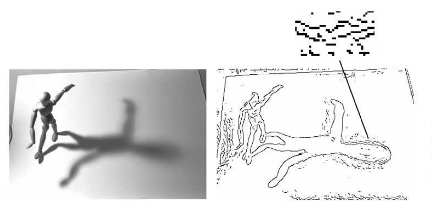
\includegraphics[width=0.8\textwidth]{capitulos/reconhecimento_borda.png}
    \caption{Exemplo de reconhecimento de bordas. Na direita: Imagem original; Na esquerda: Bordas reconhecidas pelo método de Canny/Deriche com afinamento para as bordas do manequim. Adaptado de \cite{szeliski2021computer}}
    \label{fig:reconhecimento_borda}
\end{figure}
\par
Utilizando o vetor $S_{\sigma}(X)$ deve-se calcular os cruzamentos de zero do vetor e depois realizar a conversão desses para elementos de borda. Uma forma de encontrar esses elementos é o de verificar os pixeis adjacentes $X_{i}$ e $X_{j}$ onde ocorre a troca de sinal, ou seja, $[S(X_{i}) > 0] \neq [S(X_{j} > 0]$. A localização desses pixels pode ser realizada através do cálculo do valor da intersecção em x entre a linha que existe entre $S(X_{i})$ e $S(X_{j})$ através da equação \ref{eq:borda_xintercept}. \cite{szeliski2021computer} \cite{marr1980theory}
\begin{equation}
    X_{z} = \frac{X_{i} S(X_{j}) - X_{j} S(X_{i}) }{ S(X_{j}) -  S(X_{i})}
    \label{eq:borda_xintercept}
\end{equation}
Com os cruzamentos de zero encontrados obtém-se as bordas da figura. Na literatura existem diversos algoritmos otimizados para realização dos cálculos citados acima e obtenção de uma nova imagem contendo apenas os pontos de borda.
\par
Enquanto técnicas para encontrar bordas são úteis para aplicações como reconhecimento de linha, é possível ampliar a gama de aplicações quando utilizadas junto às técnicas de geração de contorno. Contornos são definidos como a ligação entre dois pontos de borda, através deles é possível realizar a delimitação completa de uma figura, fechando o espaço entre as bordas, e a geração de uma nova imagem que represente qualitativamente a figura original. \cite{szeliski2021computer} 
\par
O jeito mais simples de criar contornos é através da ligação direta de um ponto de borda com o seu vizinho mais próximo, através de uma reta. Com o vetor de zeros em mãos é possível encontrar esses vizinhos de forma eficiente e realizar a ligação através de retas. Em caso de vizinhos ambíguos, ou seja, que possuem a mesma distância euclidiana, é possível utilizar outros parâmetros para definir qual o ponto correto de ligação, como por exemplo a direção da intensidade à qual aquele ponto é vinculado, informação obtida pela equação \ref{eq:borda_jsigma}. A técnica de ligação de pontos através de retas pode ser o bastante para alguns casos, mas é possível a obtenção de contornos mais finos através do uso de filtros e também da parametrização por arcos, permitindo a criação de contornos curvos entre dois pontos.
\begin{figure}[ht]
    \centering
    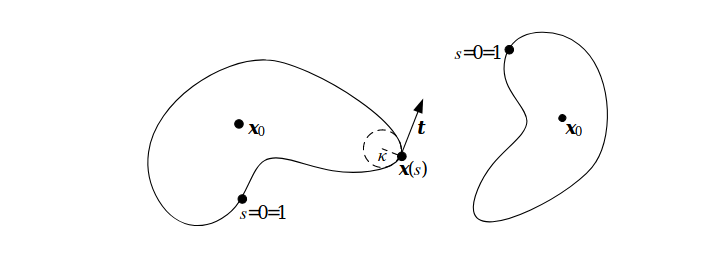
\includegraphics[width=0.8\textwidth]{capitulos/contornos_arcos.png}
    \caption{Parametrização de contornos utilizando arcos. \cite{szeliski2021computer}}
    \label{fig:contornos_arcos}
\end{figure}
\section{Planejamento de Caminhos}
Planejamento de caminhos é uma área multidisciplinar que envolve robótica, instrumentação, visão computacional e também inteligência artificial. O problema de planejamento de caminhos pode ser formulado, de maneira simplificada, por:
\begin{itemize}
    \item $ A \subset W $ : O robô, $A$ formado por uma estrutura rígida e móvel se movendo por um mundo $W$ que pode pertencer a $ \mathbb{R^2} $ ou $ \mathbb{R^3} $;
    \item $ O \subset W $ : Obstáculos rígidos e estacionários pertencentes ao mundo $W$;
    \item Tanto a geometria, a posição e a orientação de $A$ e $O$ são conhecidas a priori;
    \item A localização de $O$ em $W$ é bem conhecida.
\end{itemize}
Dado uma posição inicial e um objetivo para $A \subset W$, planejar um caminho $P \subset W$ que denota um conjunto de posições onde $ A(p)\cap O = \emptyset$ para cada posição $p \in P$ dentro do caminho que liga a posição inicial até o objetivo, retornando $P$ caso o caminho exista ou $\emptyset$ caso não exista. \cite{koubaa2018robot}
\par
De acordo com \citeonline{koubaa2018robot}, o problema de planejamento de caminhos pode ser classificado sob a visão de três grupos: o ambiente, o tipo de algoritmo e a integridade. Conforme a classificação do problema, diferentes estratégias podem ser utilizadas para resolve-lo. O ambiente pode ser dinâmico, onde o conjunto $O$ pode variar com relação ao tempo ou estático, onde o conjunto é fixo. O tipo de algoritmo pode ser local ou global, ou seja, o robô pode possuir um mapeamento fixo ou baseado em sensores e mudanças do ambiente. Já a integridade do algoritmo pode ser exata ou heurística, dependendo da necessidade de precisão do planejamento de caminho. A figura \ref{fig:pathplanning_classificacao} representa um diagrama com as classificações.
\begin{figure}[ht]
    \centering
    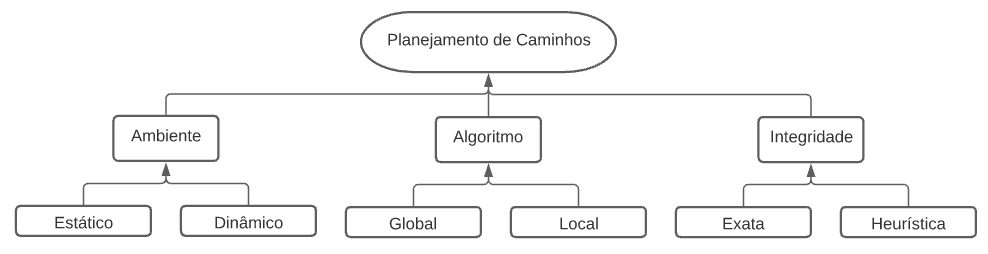
\includegraphics[width=1\textwidth]{capitulos/pathplanning_classificacao.png}
    \caption{Categorias de planejamento de caminhos. Adaptado de \cite{koubaa2018robot}}
    \label{fig:pathplanning_classificacao}
\end{figure}
\par
Existe uma variedade de algoritmos que podem ser utilizados para a solução de problemas de planejamento de caminhos. De acordo com \citeonline{latombe2012robot}, a maioria dos métodos tradicionais utiliza uma abordagem gráfica e analítica, incluindo roadmap, busca taboo, algoritmos genéticos, algoritmos de colônia e outros. Também existem algoritmos híbridos que utilizam parte exata e parte heurística e podem ser utilizados para resolução de problemas mais complexos.
\cite{koubaa2018robot}
\par
\citeonline{he2017comparison} realizaram a comparação entre quatro algoritmos de busca utilizados em plataformas de robôs móveis autônomos. O experimento levou em consideração o tempo de processamento do experimento e também o número de pontos que o experimento gerava para o caminho escolhido. Tudo isso realizado em três situação: com um obstáculo próximo ao início do percurso, com um obstáculo no final e também com três obstáculos espalhados durante o percurso.
\begin{table}[h!]
        \centering
        \caption{Tempo de Execução dos 4 Algoritmos. \cite{he2017comparison}}
        \begin{tabular}{| c | c | c | c |}
        \hline
        \textbf{Algortimo} & \textbf{Experimentos} & \textbf{Tempo de Execução (s)} & \textbf{Tempo de Execução (s)} \\
        \hline
            Dijkstra & 25 & 3.029996 & 1.01 \\
            \hline
            Floyd & 25 & 3.06997 & 1.10233 \\
            \hline
            Ant & 25 & 3.383045 & 1.1277 \\
            \hline
            A* & 25 &  3.278161 & 1.0927 \\
        \hline
        \end{tabular}
        \label{tab:pathplanning_algo4}
    \end{table}

\begin{table}[h!]
        \centering
        \caption{Tamanho dos Caminhos Encontrados para Três Obstáculos. \cite{he2017comparison}}
        \begin{tabular}{| c | c | c | c |}
        \hline
        \textbf{Algortimo} & \textbf{Três Obstáculos Fixos} & \textbf{Obstáculo Próximo ao Início} & \textbf{Obstáculo Próximo ao Fim} \\
        \hline
            Dijkstra & 1046.6 & 1046.6 & 2605.5 \\
            \hline
            Floyd & 1046.6 & 1046.6 & 2605.5  \\
            \hline
            Ant & 3869.1 & 3869.1 & 4146.6 \\
            \hline
            A* & 4023.5 &  3878.1 & 3878.1 \\
        \hline
        \end{tabular}
        \label{tab:pathplanning_algo42}
    \end{table}
    \par
    Através das tabelas \ref{tab:pathplanning_algo4} e \ref{tab:pathplanning_algo42} é possível verificar que todos os algoritmos estudados possuem um bom desempenho na solução do problema proposto, com tempo de execução próximos e diferentes respostas às situações de obstáculos. Esse tipo de comportamento permite que o desenvolvedor do sistema tenha uma grande gama de algoritmos à sua disposição para escolher. \cite{he2017comparison} 
\section{Laboratórios Remotos}
Um laboratório remoto é um tipo de laboratório virtual que, através do uso de tecnologias de software e hardware, permite que o usuário realize experimentos utilizando componentes reais de forma totalmente remota. A ideia de compartilhamento de elementos físicos através de plataformas virtuais existe desde a década de 90, quando \citeonline{aburdene1991proposal} sugere uma solução futurista para tais ambientes. \cite{ferrero2003remlab}\par
A utilização de laboratórios virtuais possui um conjunto de vantagens e desvantagens bem descritos na literatura. É comprovado que a utilização de experimentos práticos é de extrema importância em diversos níveis de ensino: técnico, graduação e também pós-graduação. Tais ferramentas O contato com o mundo real, a utilização de equipamentos reais e a compreensão de sinais reais é a única maneira de permitir que o estudante complemente a base teórica e possua uma ampla visão acerca da área de estudo. \cite{kozik2012preparing}\cite{ferrero2003remlab} 
\par
Infelizmente a realização de práticas experimentais representa o maior custo para as instituições de ensino, pois dependem de um alto investimento para aquisição e manutenção de equipamentos. Uma maneira de mitigar esse problema foi o desenvolvimento de plataformas virtuais, que necessitavam apenas de um software e servidor, para permitir que o estudantes simulem situações reais. Tal abordagem, apesar de possuir suas vantagens, não permite o contato completamente fiel à realidade e acaba por criar lacunas na aprendizagem do aluno. \cite{ferrero2003remlab} De acordo com \citeonline{sanchez2004java} não é possível substituir os experimentos in situ por simulações, mas laboratórios que utilizam a teleoperação de equipamentos reais podem ser boas alternativas para mitigar o problema dos custos de aquisição de equipamentos e do elevado número de alunos, além de permitir que as classes sejam realizadas à distância.
\par
\citeonline{sanchez2004java} também indicam que laboratórios remotos devem conseguir satisfazer três objetivos principais: educacional, organizacional e tecnológico. Por necessitar de um elevado número de tecnologias, muitas vezes a implantação desses laboratórios é realizada em parceria com empresas do setor, entretanto as instituições nas quais eles são implantados desempenham um papel fundamental para o funcionamento deles, pois as mesmas são responsáveis por realizar a preparação do material de ensino, qualificar os professores e também prover o suporte aos alunos. \cite{garcia2009addressing}
\subsection{Tipos e Classificações}

Laboratórios remotos podem ser aplicados em qualquer tipo de planta onde seja possível realizar a manipulação física do experimento e também realizar a instrumentação e processamento dos dados de forma remota. São aplicadas em diversas áreas de estudo, como: Engenharia elétrica, eletrônica, termodinâmica, fenômenos de transporte, metalurgia, mineração, robótica e estudo de estruturas. \cite{argyropoulos1983facility} \cite{sanchez2004java} \cite{andria2006remote} 
\par
Podem ser classificados de acordo com diversos parâmetros, muitas vezes essa divisão sendo realizada conforme o ponto de vista estudado pelos autores. Algumas das principais formas de classificação são:
\begin{itemize}
    \item Por finalidade: Didático ou para fins de pesquisa;
    \item Por tipo de acesso: Laboratórios de uso geral ou restrito;
    \item Pelo tipo de arquitetura utilizada: Baseado em serviços, multiplataforma, web e (ou) aplicação própria.
\end{itemize}
\subsubsection{Laboratórios Remotos via WEB}
Um dos tipos de laboratórios mais utilizados atualmente são os que possuem interface via WEB. Com a difusão da internet, aumento da tecnologia disponível nos browsers e aumento na capacidade de processamento dos computadores pessoais foi possível realizar o desenvolvimento de laboratórios que conseguem ser acessados facilmente através da maioria dos dispositivos e plataformas, sem a necessidade da instalação de nenhum software específico. \cite{andria2006remote}
\par
De acordo com \citeonline{garcia2009addressing}, o desenvolvimento de laboratórios baseados em plataforma WEB devem ser avaliados por parâmetros como segurança, acessibilidade, compatibilidade entre plataformas e dispositivos, consumo de banda e interatividade com o usuário. Esses objetivos podem ser alcançados através da utilização de boas práticas de projeto e desenvolvimento e também da escolha correta das tecnologias utilizadas, sempre visando a modernização do laboratório.
\par
A arquitetura básica de um laboratório WEB é composta por um servidor central que será responsável por realizar a comunicação com os instrumentos e também a entrega dos dados necessários para o usuário. A figura X mostra um diagrama simplificado que pode ser utilizado para representar os agentes do sistema e o papel exercido por cada um deles.
\begin{figure}[ht]
    \centering
    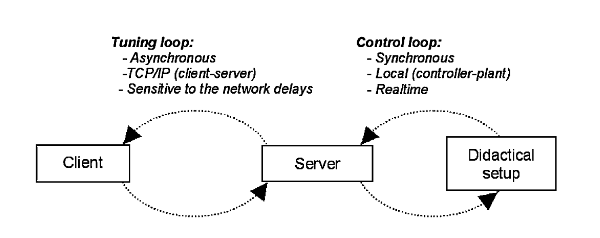
\includegraphics[width=.7\textwidth]{capitulos/servidorlaboratorio.png}
    \caption{Representação de agentes envolvidos em um laboratório remoto WEB com teleoperação. \cite{sanchez2004java}}
    \label{fig:servidorlaboratorio}
\end{figure}
\par
É importante ressaltar que o bom funcionamento de um laboratório operado via web depende do poder de processamento do servidor, da capacidade de banda disponível na instituição e de uma infraestrutura de rede robusta para garantir que a comunicação seja feita de maneira correta e em tempo real.
\chapter{Desenvolvimento}

Deve conter a descrição da área de estudo e dos materiais (banco de dados, coleta de dados, imagens, etc) e dos procedimentos metodológicos (experimentos, entrevistas, métodos estatísticos, etc) que serão empregados na realização do trabalho, de maneira que outros pesquisadores possam reproduzir o estudo. Pode ser apresentada na forma de subdivisões abaixo

\section{Caracterização da área de estudo}

\section{Dados}

\section{Metodologia}

\section{Método ou procedimento de análise A}

\section{Método ou procedimento de análise B}
\chapter{Resultados}

\chapter{Resultados}


% ELEMENTOS PÓS-TEXTUAIS
% ---------------------------------
\postextual
% ---------------------------------

% Referências
% ---------------------------------
\bibliography{abntex2-modelo-references}
% ---------------------------------

% Glossário
% ---------------------------------
%
% Consulte o manual da classe abntex2 para orientações sobre o glossário.
%
%\glossary

% ----------------------------------------------------------
% Apêndices
% ----------------------------------------------------------
%(Lembre-se: Apendices são de autoria do próprio autor do texto. 
% Anexos são elementos de autorias de outros, que o autor do texto julga interessante apresentar)
% ---
% Inicia os apêndices: 
% ---
\begin{apendicesenv}

% Insere arquivo com os apendices A e B
\chapter{Título do apêndice}

\chapter{Título do apêndice}

\end{apendicesenv}
% ---

% ------------------------------------------
% Anexos
% ------------------------------------------
%(Lembre-se: Apendices são de autoria do próprio autor do texto. 
% Anexos são elementos de autorias de outros, que o autor do texto julga interessante apresentar)
% ---
% Inicia os anexos
% ---
\begin{anexosenv}

% Insere arquivo com os anexos 1, 2 e 3
\chapter{Título do anexo}

\chapter{Título do anexo}


% ---
\end{anexosenv}

%----------------------------------
% INDICE REMISSIVO
%----------------------------------
%\phantompart
\printindex
%----------------------------------

\end{document}